%!TEX root = ../article.tex

% A new section
\section{Evaluation}
\label{sec:evaluation}
After the implementation of our Smart Places solution we performed an evaluation.
Most times the mobile apps scan for nearby beacons, they try to get the nearest one.
The code to handle the beacons has a method to get a distance from a given beacon.
Since Smart Places rely on the nearest beacon, there is a need to check if the distance value is reliable.
We performed a set of experiments in order to verify if the distance value is reliable.

The mobile app for end users keeps running in background scanning for nearby beacons, which can introduce an overhead in terms of energy comsumption.
A second set of experiments was done in order to measure the power drain of our mobile app for end users.

% Setup
In the evaluation process, a smartphone and a set of three beacons from \tm{Estimote} were used.
The smartphone was a \tm{Motorola}
Moto G\footnote{http://www.gsmarena.com/motorola\_moto\_g-5831.php}.
This device has the following specifications:
\begin{itemize}
  \item \gls{CPU}: Quad-core 1.2 GHz Cortex-A7\footnote{http://www.arm.com/products/processors/cortex-a/cortex-a7.php}
  \item \gls{GPU}: Adreno 305
  \item \gls{RAM}: 1 \gls{GB}
  \item Internal storage: 16 \gls{GB}
  \item Screen: 4.5 inches
  \item Battery: Non-removable Li-Ion 2070 \gls{mAh} battery
  \item \gls{OS}: Android 5.0.2 (Lollipop\footnote{https://www.android.com/versions/lollipop-5-0})
\end{itemize}

\subsection{Nearest Beacon Detection}
\label{sec:evaluation_nearest_beacon}
Our solution relies on a library, which its \gls{API} allows us to get the distance from a given beacon.
However, this value is related to the signal's strength, that comes from the beacon.
We performed a set of experiments to verify how reliable was this value and if we can use that value to compute which beacon is the nearest one.

% Nearest Beacon: Methodology
The set of experiments, is summarized in Table~\ref{tab:experiments_nearest_beacon}.
Figure~\ref{fig:layout_experiments_nearest_beacon} shows the layout that was used where value d is the distance between beacons.
In these experiments, the Smart Musem example was used.
In each experiment, it ran for 5 minutes using 10 seconds as the interval between each scan.
10 seconds was chosen because it is a reasonable value to walk in the museum to have enough time to perform any computation, that was needed, after each scan.
Running the experiment for 5 minutes, with the mentioned interval between each scan, allowed us to have more than 20 scans.
Then, in Android Studio log output, it was possible to check how many times each beacon was detected as the nearest one.

\begin{table}[]
\centering
\begin{tabular}{@{}|l|c|c|c|c|@{}}
\toprule
\multicolumn{1}{|c|}{}                & \multicolumn{4}{c|}{{\bf Experiments}}                                                                            \\ \midrule
\multicolumn{1}{|c|}{{\bf Variables}} & {\bf 1}                     & {\bf 2}                   & {\bf 3}                     & {\bf 4}                   \\ \midrule
Events                                & \multicolumn{4}{c|}{\begin{tabular}[c]{@{}c@{}}For each beacon, \\ how many times \\ it was scanned\end{tabular}} \\ \midrule
Number of beacons                     & \multicolumn{4}{c|}{3}                                                                                            \\ \midrule
Interval between each scan (seconds)  & \multicolumn{4}{c|}{10}                                                                                           \\ \midrule
Experiment duration (minutes)         & \multicolumn{4}{c|}{5}                                                                                            \\ \midrule
Distance between beacons (meters)     & \multicolumn{1}{r|}{0.5}    & \multicolumn{1}{r|}{1}    & \multicolumn{1}{r|}{1.5}    & \multicolumn{1}{r|}{2}    \\ \bottomrule
\end{tabular}
\caption[Nearest beacon experiments summary]{Experiments to get the accuracy of the method to get the nearest beacon}
\label{tab:experiments_nearest_beacon}
\end{table}


\begin{figure}[!ht]
  \centering
    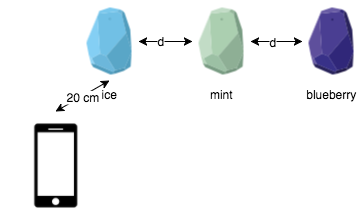
\includegraphics[width=0.4\textwidth, keepaspectratio]{figures/nearest_beacon}
    \caption[Layout for experiments of nearest beacon]{Layout used for the experiments to get the accuracy of the distance value}
    \label{fig:layout_experiments_nearest_beacon}
\end{figure}

% Nearest beacon: Results
The mobile app for end users scans for beacons but only requests data for the nearest one. To get the nearest one, it has to rely on the signal strength to calculate the distance. We performed 4 experiments in order to try to get the accuracy of the mechanism that calculates the distance that the mobile device is from a given beacon.

For each experiment, we counted how many times each beacon was detected as the nearest one.
Looking at the layout used in these experiments we can see that the app should detect the beacon named \emph{ice} as the nearest one.
Figure~\ref{fig:results_experiments_nearest_beacon} shows the percentage of times that the beacon \emph{ice} was detected as the nearest one, showing that, as we increase the distance between beacons, the accuracy to detect the nearest beacon also increases.
From the results, we can conclude that it is recommended that the beacons are, at least, 1.5m or 2m distant from each other.

\begin{figure}[!ht]
  \centering
    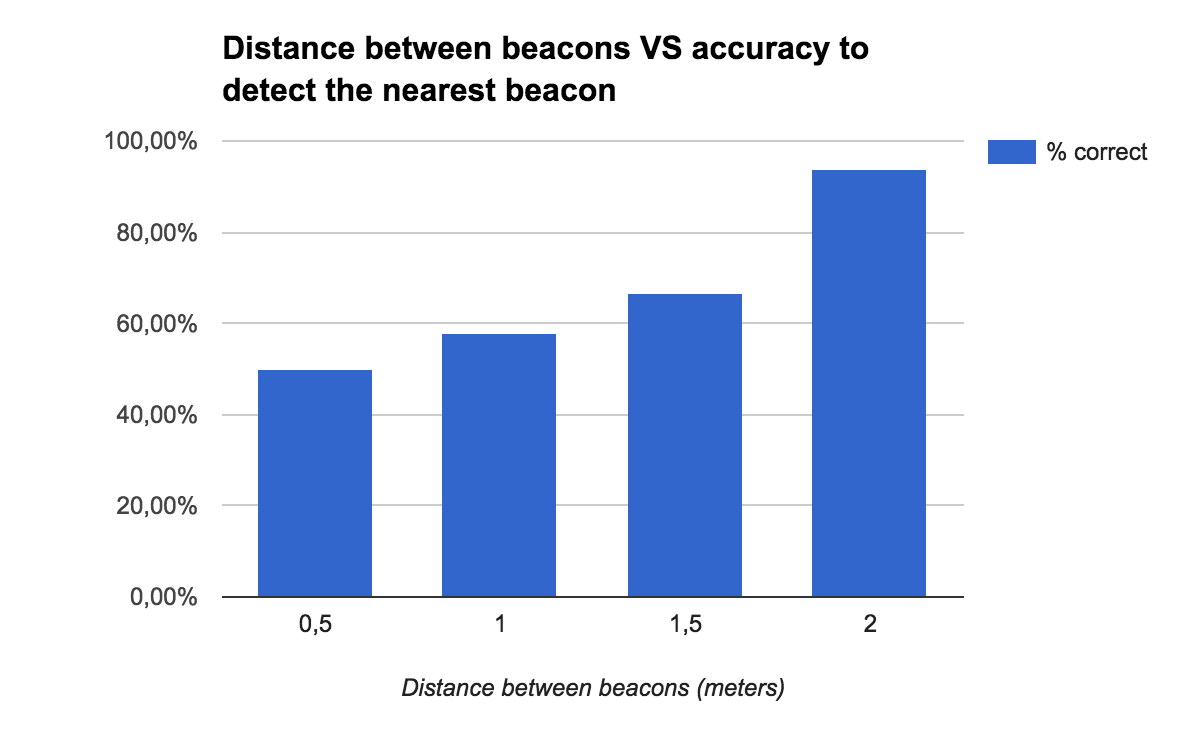
\includegraphics[width=0.5\textwidth, keepaspectratio]{figures/results_nearest_beacon}
    \caption[Distance between beacons vs Accuracy]{Relation between distance between beacons and accuracy to detect the nearest beacon}
    \label{fig:results_experiments_nearest_beacon}
\end{figure}

In an environment, where the beacons are close to each other, our solution might not work as expected.
For instance, in the previously described Smart Restaurant example,
the tables should not be close to each other. This is not always possible because, some restaurants try to optimize space and have tables as much close to each other as possible.
In the Smart Museum example, two objects, in a given exhibition, should not be close to each other.
Otherwise, the visitor would be notified about an object and he might be looking at another one.

% Energy Comsumption
\subsection{Energy Consumptions}
\label{sub:evaluation_energy_consumptions}
Another important aspect of this solution is the battery consumption.
Since our mobile app for end users runs on background to scan for nearby beacons, that can have a negative impact on the device's battery. If the user notice that the battery drains too fast, he/she will not use this solution.

% Energy consumption
Table~\ref{tab:experiments_battery} summarizes the experiments performed to evaluate the battery consumption.
Figure~\ref{fig:layout_experiments_battery_consumption} shows the layout used for this group of experiments.
The beacons are equally distant, 25 cm, from each other.
The smartphone is at the same distance from the beacon in the middle, the green one named mint.
We performed six experiments.
In each one the app was turned on and ran for 1 hour, in background mode, scanning for beacons in order to discover nearby Smart Places.
The first two used \gls{WiFi} data connection.
The remaining used \gls{3G} mobile network.
Different data connection means can lead to different energy consumptions.
We need to understand which connection, \gls{WiFi} or \gls{3G}, drains more power.
If it is \gls{3G}, the user might only use our solution if he/she is connected to a \gls{WiFi} \gls{AP}.
We want our mobile app to be always turned on scanning for nearby Smart Places.
Using it only when \gls{WiFi} is available would make its usage very limited and the user would not take the full advantage of it, because he/she needs be aware that a \gls{WiFi} \gls{AP} is available and turn the mobile app on again.
We tested two values for the interval between each scan, 5 minutes, because it is the default value that the beacons library use in background mode, and 2 and half minutes.
The second value is half the first in order to see how much more power is drained when we set a smaller value for the interval between each scan.
Trying to find a smaller interval is important because it will reduce the probability that the user was not able to discover a nearby Smart Place.

The following scenarios were tested:
\begin{itemize}
  \item
  When the user stays in the same Smart Place the entire experiment;
  \item
  When the user moves from one Smart Place to another, at each two and half minutes.
  This is done removing existing data about Smart Places already detected to force the app to request this data again from the Backend.
\end{itemize}

% Please add the following required packages to your document preamble:
% \usepackage{booktabs}
\begin{table}[]
\centering
\begin{tabular}{@{}|c|c|c|c|c|@{}}
\toprule
\multicolumn{1}{|l|}{}                     & \multicolumn{4}{c|}{{\bf Experiments}}                                                                \\ \midrule
{\bf Variables}                            & {\bf 1}                  & {\bf 2}                & {\bf 3}                  & {\bf 4}                \\ \midrule
{\bf Data connection type}                 & \multicolumn{2}{c|}{WiFi}                         & \multicolumn{2}{c|}{3G}                           \\ \midrule
{\bf Interval between each scan (minutes)} & \multicolumn{1}{r|}{2.5} & \multicolumn{1}{r|}{5} & \multicolumn{1}{r|}{2.5} & \multicolumn{1}{r|}{5} \\ \midrule
{\bf Experiment duration (hours)}          & \multicolumn{4}{c|}{1}                                                                                \\ \bottomrule
\end{tabular}
\caption[Battery consumption results]{Summary of experiments to get the battery consumption when the mobile
app is scanning for beacons in the background}
\label{tab:experiments_battery}
\end{table}


\begin{figure}[!ht]
  \centering
    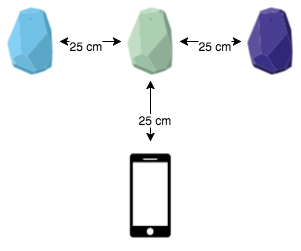
\includegraphics[width=0.3\textwidth, keepaspectratio]{figures/experiments_battery_layout}
    \caption[Layout for experiments of battery consumption]{Layout used for the experiments to get the battery consumption}
    \label{fig:layout_experiments_battery_consumption}
\end{figure}

Data communications, \gls{WiFi} or \gls{3G}, are the major source of battery drain, as suggested in studies, such as \cite{energy}.
We used Battery Historian\footnote{https://developer.android.com/tools/performance/batterystats-battery-historian/index.html} to measure the power drain and how much data was transferred (sent and received).

% Energy Consumption: Results
Figure~\ref{fig:results_battery_stopped} shows the results for the first scenario, where the user does not move.
The battery consumption using \gls{WiFi} are almost zero.
However, when using \gls{3G}, the battery consumption raises more than 30 times than using \gls{WiFi}.
The battery consumption using \gls{WiFi} is almost zero.
However, when using \gls{3G}, the battery consumption raises more than 30 times than using \gls{WiFi}.

\begin{figure}[!ht]
  \centering
    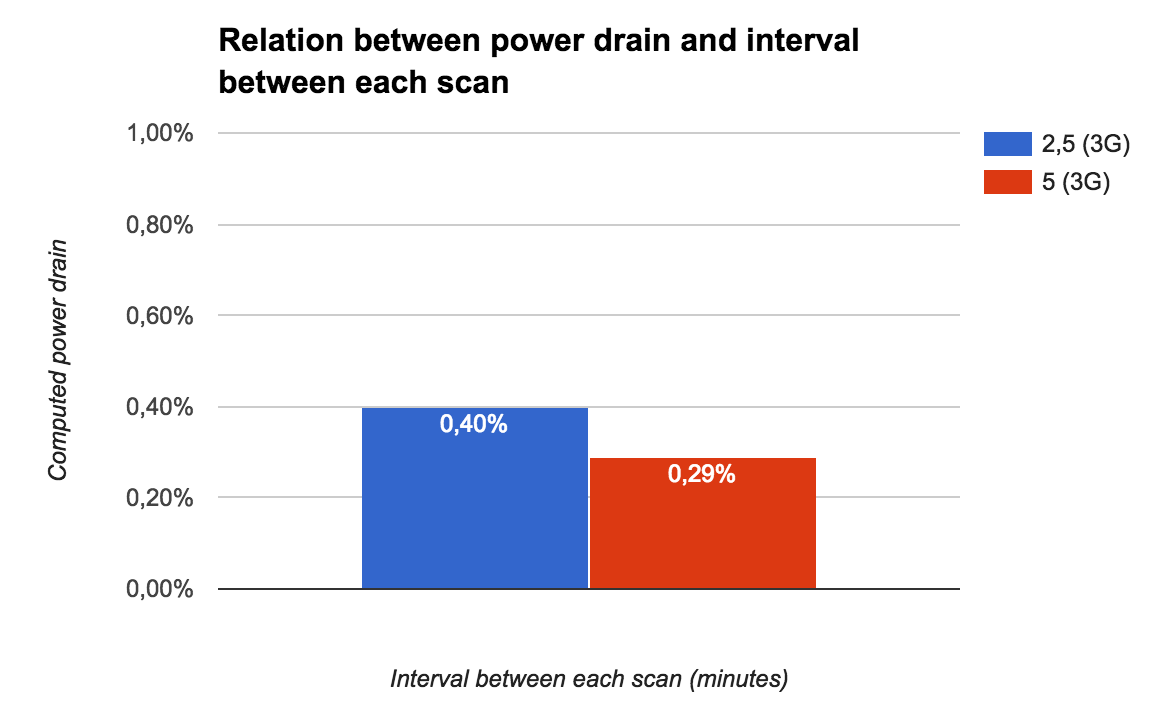
\includegraphics[width=0.5\textwidth, keepaspectratio]{figures/results_battery_stopped}
    \caption[Power drain when the user does not move]{Relation between power drain and interval between each scan in the scenario where the user stays in the same Smart Place}
    \label{fig:results_battery_stopped}
\end{figure}

From this results, it is possible to conclude that, our solution, introduces the most overhead when using \gls{3G} as the mean to perform data communications, such as, communications with the backend.
For each data connection type (\gls{WiFi} and \gls{3G}), we tested two values for the interval between each scan for nearby beacons.
We can observe, when we decrease the interval between each scan in half, the battery consumption increases in 0.1\%.
Taking into account that we spent one hour, in each experiment, assuming that the values, for the power drain, grow lineary, it is possible to say that, for two and half and five minutes, in interval between each scan, we would have 6.96\% and 9.6\%, in 24 hours, of power drain, respectively.
The values are still low but these values can demotivate the usage of our solution because, it is very likely that the users already have mobile apps, that use mobile data, already installed in their devices.

Regarding the second scenario, where the user moves from one Smart Place to another, Figure~\ref{fig:results_battery_walking} shows more power drain than in the previous scenario.
Once more, we have much more power drain using \gls{3G}.
Using two minutes and half of interval between each scan, we got more 0.71\% than using five minutes.
Assuming a linear growth of power drain, in the worst case, after 24 hours, there is 65.04\% of power drain.
In this case, we got more than 60 times the power drain than the worst case in the previous scenario.
With this value, our solution can be considered unacceptable for a daily basis usage, that is, having the mobile app always running in background.

\begin{figure}[!ht]
  \centering
    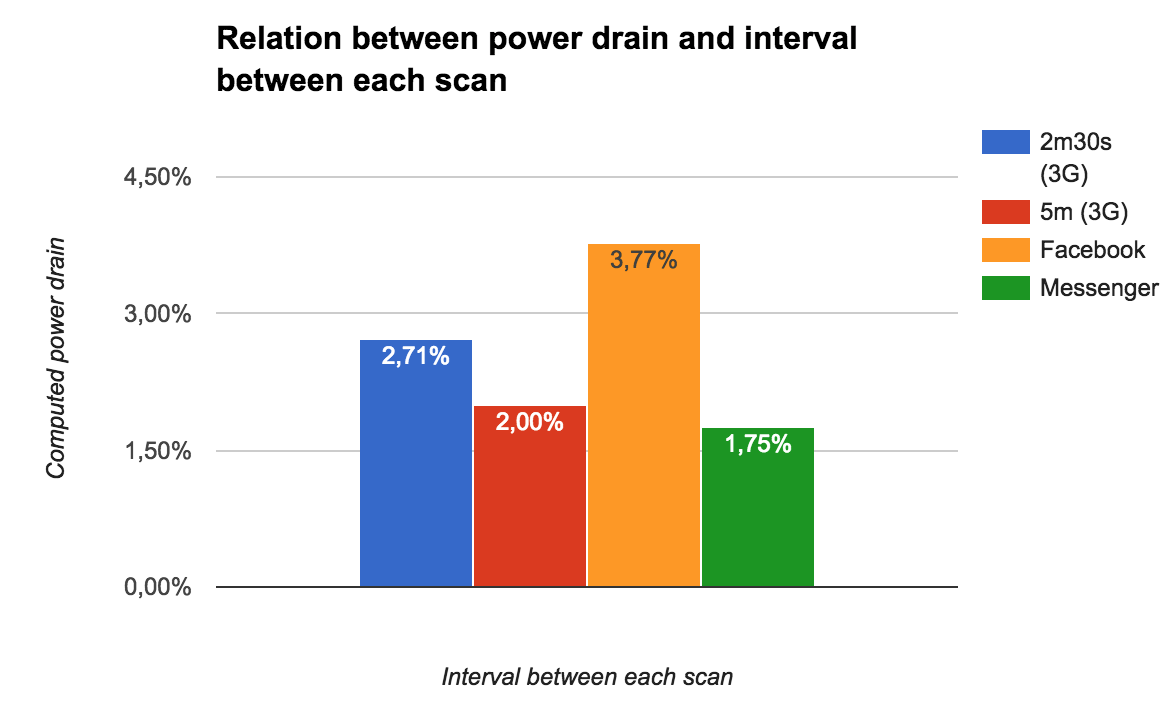
\includegraphics[width=0.5\textwidth, keepaspectratio]{figures/results_battery_walking}
    \caption[Power drain when the user is moving]{Relation between power drain and interval between each scan in the scenario where the user moves along multiple Smart Places}
    \label{fig:results_battery_walking}
\end{figure}

In the worst case, which is the user is always moving, the results can compromise the usability of our solution because, assuming a linear growth of power drain, in 24 hours, our mobile app would drain 48\%.
Having into account that most users already have apps that require a data connection, this can be unnaceptable in most cases.
